\documentclass{article}
\usepackage[utf8]{inputenc}
\usepackage{latexsym} 
\usepackage{amssymb,amsmath} 
\usepackage{tikz}
\usetikzlibrary{shapes,arrows,positioning }
\usepackage[english]{babel}
\usepackage{biblatex}
\usepackage{mathtools}
\usepackage{xcolor}
\usepackage{comment}
\newcommand\Myperm[2][^n]{\prescript{#1\mkern-2.5mu}{}P_{#2}}
\setcounter{tocdepth}{4}
\setcounter{secnumdepth}{4}
                
\title{STAT 110 HW 10}
\author{Moses Stewart}
\date{November 2022}

\begin{document}
\maketitle

\subsection{Problem 1}
We are given that $P(L(X) < \theta < U(X)) = 0.95$, and that there are $n$ frequentists where the $j^{\text{th}}$ frequentists observes data $X_{j}$ and makes a confidence interval for the parameter $\theta_{j}$. We want to show that as $n \rightarrow \infty$, the fraction of the intervals which contain the parameter $\rightarrow 0.95$.

Now, let:
$$I_{j} = I(L(X_{j}) < \theta_{j} < U(X_{j}))$$
for the $j^{\text{th}}$ frequentist, where $P(I_{j}) = 0.95$ based on the condition given in the problem.

Additionally, let:
$$R_{n} = I_{1} + I_{2} + ... + I_{n}$$
count the number of frequentists whose confidence interval contained $\theta_{j}$. Since the indicators are bernoulli with a probability of success $P(I_{j}) = 0.95$, we know that $R_{n} \sim \text{Bin}(n, 0.95)$.

This means that by definition, the expectation of $R_{n}$ is given by:
$$E(R_{n}) = 0.95n$$
and the sample mean of each $I_{1}, I_{2}, ..., I_{n}$ is given by:
$$\overline{I_{j}} = \frac{R_{n}}{n}$$
 
Because $R_{n}$ is the sum of $I_{1}, I_{2}, ..., I_{n}$ i.i.d. indicators with $P(I_{j}) = 0.95$, the law of large numbers tells us that with probability 1, the sample mean for each $\overline{I_{j}} = \frac{R_{n}}{n} \rightarrow 0.95 = P(I_{j})$ as $n \rightarrow \infty$.

\subsection{Problem 2}
\subsubsection{Part a}
We are given that a hedge fund manager always invests half of her fortune into the stock each day. $Y_{n}$ is her fortune after $n$ days, starting from an initial fortune of $Y_{0} = 100$. We are asked what happens to $Y_{n}$ as $n \rightarrow \infty$.

Let $U_{n}$ be the number of times the stock increases in a period of $n$ days. Because the hedge fund manager invests half of her fortune each day, on day $n = 1$ if the stock price increases:
$$Y_{1} = \frac{Y_{0}}{2} + \frac{Y_{0}}{2}(1.7) = 1.35Y_{0}$$
If the stock price decreases:
$$Y_{1} = \frac{Y_{0}}{2} + \frac{Y_{0}}{2}(0.5) = 0.75Y_{0}$$

This means that every time the stock goes up, her fortune increases by $1.35$ fold, and every time the stock goes down her fortune increases by $0.75$ fold. Therefore, we can write a general equation:
$$Y_{n} = Y_{0}(1.35)^{U_{n}}(0.75)^{n - U_{n}}$$

We can simplify this using exponent rules to find that:
$$Y_{n} = Y_{0}\bigg[\bigg(\frac{1.35}{0.75}\bigg)^{\frac{U_{n}}{n}}0.75\bigg]^{n} = Y_{0}\bigg[(1.8)^{\frac{U_{n}}{n}}0.75\bigg]^{n}$$

To find what happens to $Y_{n}$ as $n \rightarrow \infty$, we can take the limit of each side:
$$\lim_{n \rightarrow \infty}Y_{n} = \lim_{n \rightarrow \infty} Y_{0}\bigg[(1.8)^{\frac{U_{n}}{n}}0.75\bigg]^{n}$$

By the law of large numbers, because $\frac{U_{n}}{n}$ is the sample mean of how many times the stock goes up, as $n \rightarrow \infty$, $\frac{U_{n}}{n} \rightarrow \frac{1}{2}$

$$\Rightarrow \lim_{n \rightarrow \infty}Y_{n} = \lim_{n \rightarrow \infty} Y_{0}\bigg[(1.8)^{\frac{1}{2}}0.75\bigg]^{n}$$

$$\lim_{n \rightarrow \infty}Y_{n} = \lim_{n \rightarrow \infty} Y_{0}[1.006]^{n}$$
$$\lim_{n \rightarrow \infty}Y_{n} = \infty$$

\subsubsection{Part b}
We are given that the hedge fund manager invests a fraction $\alpha$ of her current fortune each day, and are asked to find the function $g(\alpha)$ such that:
$$\frac{\text{log}Y_{n}}{n} \rightarrow g(\alpha)$$
with probability $1$ as $n \rightarrow \infty$.

First, to find a function for what $\frac{\text{log}Y_{n}}{n}$ approaches as $n \rightarrow \infty$ in terms of $\alpha$, we first want to find a function $Y_{n}$ in terms of $\alpha$.

By definition, if her stock goes up, the hedge fund manager will gain $\alpha \times 1.7$ her current fortune, and the remaining $(1 - \alpha)$ portion of her fortune that she didn't invest will remain. Therefore, every time her stock increases her fortune will increase by:
$$(1.7)\alpha + (1 - \alpha) = 0.7\alpha + 1$$
By the same logic, if her stock goes down, the hedge fund manager will lose the $\alpha \times 0.5$ her current fortune, nd the remaining $(1 - \alpha)$ portion of her fortune that she didn't invest will remain. Therefore, every time her stock increases her fortune will decrease by:
$$(0.5)\alpha + (1 - \alpha) = -0.5\alpha + 1$$

Plugging this into our original equation for $Y_{n}$ in place of the ratios we had for part a, we find that:
$$Y_{n} = Y_{0}(0.7\alpha + 1)^{U_{N}}(-0.5\alpha + 1)^{n - U_{N}}$$
$$\text{log}Y_{n} = \text{log}Y_{0} + U_{n} \text{log}(0.7\alpha + 1) + n \text{log}(-0.5\alpha + 1) - U_{n} \text{log}(-0.5\alpha + 1)$$
$$\text{log}Y_{n} = \text{log}Y_{0} + U_{n} \text{log}(\frac{0.7\alpha + 1}{-0.5\alpha + 1}) + n \text{log}(-0.5\alpha + 1))$$
$$\frac{\text{log}Y_{n}}{n} = \frac{\text{log}Y_{0}}{n} + \frac{U_{n}}{n} \text{log}(\frac{0.7\alpha + 1}{-0.5\alpha + 1}) + \text{log}(-0.5\alpha + 1))$$

Now, to find $g(\alpha)$ as $n \rightarrow \infty$, we can take the limit of both sides:
$$\lim_{n \rightarrow \infty} \frac{\text{log}Y_{n}}{n} = \lim_{n \rightarrow \infty} \frac{\text{log}Y_{0}}{n} + \frac{U_{n}}{n} \text{log}(\frac{0.7\alpha + 1}{-0.5\alpha + 1}) + \text{log}(-0.5\alpha + 1))$$

By the law of large numbers, because $\frac{U_{n}}{n}$ is the sample mean of how many times the stock goes up, as $n \rightarrow \infty$, $\frac{U_{n}}{n} \rightarrow \frac{1}{2}$

$$\Rightarrow \lim_{n \rightarrow \infty} \frac{\text{log}Y_{n}}{n} = 0 + \frac{1}{2} \text{log}(\frac{0.7\alpha + 1}{-0.5\alpha + 1}) + \text{log}(-0.5\alpha + 1))$$
$$\lim_{n \rightarrow \infty} \frac{\text{log}Y_{n}}{n} = \frac{1}{2} \text{log}(0.7\alpha + 1) + \frac{1}{2}\text{log}(-0.5\alpha + 1))$$
$$\lim_{n \rightarrow \infty} \frac{\text{log}Y_{n}}{n} = \frac{1}{2} \text{log}[(0.7\alpha + 1)(-0.5\alpha + 1)]$$
Therefore:
$$\frac{\text{log}Y_{n}}{n} \rightarrow g(\alpha) = \frac{1}{2} \text{log}[(0.7\alpha + 1)(-0.5\alpha + 1)]$$
With probability 1 as $n \rightarrow \infty$

A log function is strictly increasing over its entire domain, so to find where $g(\alpha)$ is maximized, we can calculate where $(0.7 \alpha + 1)(-0.5 \alpha + 1)$ is maximized. Doing so, we find:

$$g(\alpha) = \frac{1}{2} \text{log}[-\frac{7}{20}\alpha^{2} + \frac{1}{5}\alpha + 1]$$
$$g(\alpha) = \frac{1}{2} \text{log}[-\frac{7}{20}(\alpha^{2} - \frac{4}{7}\alpha + \frac{4}{49} - \frac{144}{49}]$$
$$g(\alpha) = \frac{1}{2} \text{log}[-\frac{7}{20}(\alpha - \frac{2}{7})^{2} + \frac{36}{35}]$$

The function $-\frac{7}{20}(\alpha - \frac{2}{7})^{2} + \frac{36}{35}$ is clearly a concave quadratic with a vertex at $\frac{2}{7}$, so we can conclude that that is where $g(\alpha)$ is maximized.

\subsection{Problem 3}
\subsubsection{Part a}
We are trying to estimate $\theta$ based on data $X_{1}, X_{2}, ..., X_{n}$, where $T_{1}$ is a function of $X_{1}, X_{2}, ..., X_{n}$ used to estimate $\theta$ and $T_{2} = E(T_{1}|R)$. We are trying to show that:
$$E(T_{2} - \theta)^{2} < E(T_{1} - \theta)^{2}$$

We can simplify the right side of the equation to find that:
$$E(T_{1} - \theta)^{2} = E(T_{1}^{2} - 2T_{1}\theta + \theta^{2})$$
$$E(T_{1} - \theta)^{2} = E(T_{1}^{2}) - E(2T_{1}\theta) + E(\theta^{2})$$

In this problem, both $2$ and $\theta$ are treated as constants. Therefore:
$$E(T_{1} - \theta)^{2} = E(T_{1}^{2}) - 2\theta E(T_{1}) + \theta^{2}$$
Using Adam's law, we find:
$$E(T_{1} - \theta)^{2} = E(E(T_{1}^{2}|R)) - 2\theta E(E(T_{1}|R)) + \theta^{2}$$
We are given that $T_{2} = E(T_{1}|R)$, so we know that $T_{2}^{2} = E(T_{1}|R)^{2}$. Now, $T_{1}^2$ is a convex function. Therefore, by Jenson's inequality, we can conclude that:
$$T_{2}^{2} = E(T_{1}|R)^{2} \leq E(T_{1}^{2}|R)$$

Therefore:
$$E(T_{1} - \theta)^{2} \geq E(T_{2}^{2}) - 2\theta E(T_{2}) + \theta^{2}$$

Again, $\theta$ is just a constant, so we can pull it inside the inequality.
$$E(T_{1} - \theta)^{2} \geq E(T_{2}^{2} - 2\theta T_{2} + \theta^{2})$$
$$E(T_{1} - \theta)^{2} \geq E(T_{2} - \theta)^{2}$$


\subsubsection{Part b}
We are given that the \textit{bias} of an estimator $T$ for $\theta$ is defined to be $b(T) = E(T) - \theta$. We also know that the \textit{bias-variance tradeoff} is given by:
$$E(T - \theta)^{2} = \text{Var}(T) + (b(T))^{2}$$

To give an alternative proof for part a, it suffices to show that the mean squared error $E(T_{1} - \theta)^{2}$ is greater than $E(T_{2} - \theta)^{2}$ using the equation above. First, notice that using Adam's law:
$$b(T_{1}) = E(T_{1}) - \theta$$
$$b(T_{1}) = E(E(T_{1}|R)) - \theta$$
$$b(T_{1}) = E(T_{2}) - \theta$$
$$b(T_{1}) = b(T_{2})$$

Therefore, $(b(T_{1}))^{2} = (b(T_{2}))^{2}$. This means to prove that $E(T_{1} - \theta)^{2}$ is greater than $E(T_{2} - \theta)^{2}$, using the equation above, it suffices to show that:
$$\text{Var}(T_{1}) > \text{Var}(T_{2})$$

Using EVE's law, we find that:
$$\text{Var}(T_{1}) = E(\text{Var}(T_{1}|R)) + \text{Var}(E(T_{1}|R))$$
By definition, we are given that $E(T_{1}|R) = T_{2}$, therefore:
$$\text{Var}(T_{1}) = E(\text{Var}(T_{1}|R)) + \text{Var}(T_{2})$$
$$\text{Var}(T_{1}) - E(\text{Var}(T_{1}|R)) = \text{Var}(T_{2})$$

By definition, variance is always positive, therefore $E(\text{Var}(T_{1}|R))$ must be positive. Thus, for all $T_{1}, T_{2}$:
$$\text{Var}(T_{1}) > \text{Var}(T_{2})$$
Now, because the mean squared error: $E(T - \theta)^{2} = \text{Var}(T) + (b(T))^{2}$, and $(b(T_{1}))^{2} = (b(T_{2}))^{2}$, this means that:
$$E(T_{2} - \theta)^{2} < E(T_{1} - \theta)^{2}$$

\subsubsection{Part c}
We are given that $X_{1}, X_{2}, . . .$ are i.i.d. with mean $\theta$, $T_{1} = X_{1}$, and $R = \sum_{j = 1}^{n} X_{j}$. We are asked to find $T_{2}$, check that it has a lower mean squared error than $T_{1}$ for $n \geq 2$, and say what happens to $T_{1}$ and $T_{2}$ as $n \rightarrow \infty$.

We are given that $T_{2} = E(T_{1}|R)$, so to find $T_{2}$ we need to find $E(T_{1}|R)$. We are also given that $T_{1} = X_{1}$, therefore:
$$T_{2} = E(T_{1}|R) = E(X_{1}|R)$$

To find $E(X_{1}|R)$, notice that $R = \sum_{j = 1}^{n} X_{j}$. Therefore, we know by LOTUS that:
$$E(R) = \sum_{j = 1}^{n} E(X_{j})$$
$$R = \sum_{j = 1}^{n} E(X_{j}|R)$$
Because $X_{j}$ are i.i.d., this means that:
$$R = nE(X_{1}|R)$$
$$E(X_{1}|R) = \frac{R}{n} = T_{2}$$

Now that we found $T_{2}$, we want to check that it has a lower mean squared error than $T_{1}$ for $n \geq 2$. Using the equation from part b, we find that:
$$E(T_{2} - \theta)^{2} = \text{Var}(T_{2}) + (b(T_{2}))^{2}$$
We showed in part b that $(b(T_{2}))^{2} = (b(T_{1}))^{2}$, therefore we can simplify this to:
$$E(T_{2} - \theta)^{2} = \text{Var}(\frac{R}{n}) + (E(T_{1}) - \theta)^{2}$$
$T_{1}$ is an estimator for $\theta$, therefore by definition $E(T_{1}) = \theta$, so $(E(T_{1}) - \theta)^{2} = 0$. Thus, we find:
$$E(T_{2} - \theta)^{2} = \text{Var}(\frac{R}{n})$$
$$E(T_{1} - \theta)^{2} = \text{Var}(T_{1}) = \text{Var}(X_{1})$$

Now, $n$ is a constant, so we can simplify the top equation to:
$$E(T_{2} - \theta)^{2} = \frac{\text{Var}(R)}{n^{2}}$$
Again, recall that $R = \sum_{j = 1}^{n} X_{j}$ where $X_{j}$ are i.i.d. Therefore, using the properties of variance and covariance:
$$\text{Var}(R) = \sum_{j = 1}^{n} \text{Var}(X_{j})$$
$$\text{Var}(R) = n \text{Var}(X_{1})$$
$$\Rightarrow E(T_{2} - \theta)^{2} = \frac{n\text{Var}(X_{1})}{n^{2}}$$
$$E(T_{2} - \theta)^{2} = \frac{\text{Var}(X_{1})}{n}$$

$n$ is always a positive constant, therefore:
$$\frac{\text{Var}(X_{1})}{n} < \text{Var}(X_{1})$$
Therefore because $E(T_{2} - \theta)^{2} = \frac{\text{Var}(X_{1})}{n}$ and $E(T_{1} - \theta)^{2} = \text{Var}(X_{1})$ we can conclude that:
$$E(T_{2} - \theta)^{2} < E(T_{1} - \theta)^{2}$$

Finally, $T_{1}$ is defined to be $X_{1}$, so as $n \rightarrow \infty$ $T_{1} \rightarrow X_{1}$ because $X_{1}$ does not depend on $n$. 

However, $T_{2} = \frac{R}{n}$, which is the sample mean for $\sum_{j = 1}^{n} X_{j}$. Therefore, by the law of large numbers,  as $n \rightarrow \infty$, $T_{2} \rightarrow \mu$, where $\mu$ is the true mean of $X_{1}, ..., X_{n}$.

\subsection{Problem 4}
\subsubsection{Part a}
We are given that each page of an $n$-age book has a $\text{Pois}(\lambda)$ number of typos. The number of typos on each page are i.i.d. $X_{1}, ... , X_{n} \sim \text{Pois}(\lambda)$. The probability that a page has no typos is given by $P(X_{j} = 0) = \theta = e^{-\lambda}$.

We are asked to show that $T_{n} = e^{-\overline{X}_{n}}$ is biased for estimating $\lambda$, or that $E(T_{n}) \neq \theta$. By definition, we know that:
$$E(T_{n}) = E(e^{-\overline{X}_{n}})$$

Notice that $E(e^{-\overline{X}_{n}})$ is a function of $\overline{X}_{n}$, and that $\frac{d^{2}}{dx}e^{-x} = e^{-x}$, therefore $e^{-\overline{X}_{n}}$ is a convex function. Therefore, by Jensen's inequality, this tells us that:
$$E(T_{n}) = E(e^{-\overline{X}_{n}}) \geq e^{-E(\overline{X}_{n})}$$

Because $\overline{X}_{n}$ is the sample mean for i.i.d. variables with mean $\lambda$, we know that $E(\overline{X}_{n}) = \lambda$, therefore this gives us that:
$$E(T_{n})  \geq e^{-\lambda}$$
which shows that in general $T_{n}$ is biased for estimating $\theta$.
\subsubsection{Part b}
$\overline{X}_{n}$ is the sample mean for i.i.d. $X_{i}$, and is given by:
$$\overline{X}_{n} = \frac{X_{1} + X_{2} + ... + X_{n}}{n}$$

By the law of large numbers, as $n \rightarrow \infty$, $\overline{X}_{n} \rightarrow \lambda = E(X_{i})$. Therefore, because $T_{n}$ is given by:
$$T_{n} = e^{-\overline{X}_{n}}$$
By the law of large numbers, we can conclude that with probability 1, as $n \rightarrow \infty$:
$$T_{n} \rightarrow e^{-\lambda} = \theta$$

\subsubsection{Part c}
To show that $W = \frac{1}{n} (I(X_{1} = 0) + ... + I(X_{n} = 0))$ is unbiased for $\lambda$, we want to show that $E(W) = \lambda$. Additionally, we are given that $X_{1} | (X_{1} + ... + X_{n} = s) \sim \text{Bin}(s, \frac{1}{n})$. Calculating $E(W)$:

$$E(W) = E(\frac{1}{n} (I_{1} + ... + I_{n}))$$
$$E(W) = \frac{1}{n}E(I_{1} + ... + I_{n})$$
$$E(W) = \frac{1}{n}[E(I_{1}) + ... + E(I_{n})]$$
$$E(W) = \frac{1}{n}[n P(I_{1})]$$

We know that $I_{1}$ is the event that $X_{1} = 0$, therefore:
$$P(I_{1}) = P(X_{1} = 0)$$
$$P(I_{1}) = e^{-\lambda}$$
Thus, we find:
$$E(W) = \frac{1}{n}[n e^{-\lambda}] = e^{-\lambda}$$
Therefore, $E(W) = \theta$, so $W$ is unbiased for estimating $\lambda$.
\\
\\
Now, we are asked to find $E(W| (X_{1} + ... + X_{n} = s))$. Solving, we find:
$$E(W| (X_{1} + ... + X_{n} = s)) = E(I_{1} + ... + I_{n} | (X_{1} + ... + X_{n} = s))$$
$$E(W| (X_{1} + ... + X_{n} = s)) = E(I_{1} | (X_{1} + ... + X_{n} = s) ) + ... + E(I_{n} | (X_{1} + ... + X_{n} = s))$$
$$E(W| (X_{1} + ... + X_{n} = s)) = nP(I_{1} | (X_{1} + ... + X_{n} = s) )$$
Here, we are given that $X_{1} | (X_{1} + ... + X_{n} = s) \sim \text{Bin}(s, \frac{1}{n})$. 
$$P(X_{1} = x | (X_{1} + ... + X_{n} = s)) = {s \choose x}\bigg(\frac{1}{n}\bigg)^{x}\bigg(\frac{n - 1}{n}\bigg)^{s - x}$$
$$P(X_{1} = 0 | (X_{1} + ... + X_{n} = s)) = \bigg(\frac{n - 1}{n}\bigg)^{s}$$
$$P(X_{1} = 0 | (X_{1} + ... + X_{n} = s)) = \bigg(\frac{n - 1}{n}\bigg)^{s}$$
Recall that $I_{i}$ is the indicator that page $i$ has zero typos. Therefore:
$$P(I_{1} | (X_{1} + ... + X_{n} = s)) = \bigg(\frac{n - 1}{n}\bigg)^{s}$$

Plugging this back in, we find:
$$E(W| (X_{1} + ... + X_{n} = s)) = \bigg(\frac{n - 1}{n}\bigg)^{s}$$
\\\\
Now, we are asked if $\tilde{W} = E(W| (X_{1} + ... + X_{n} = s))$ is unbiased for $\theta$. Taking the expected value of both sides:
$$E(\tilde{W}) = E(E(W| (X_{1} + ... + X_{n} = s)))$$
This is precisely defined by Adam's law, so we can easily conclude that:
$$E(\tilde{W}) = E(E(W| (X_{1} + ... + X_{n} = s))) = E(W) = e^{-\lambda}$$

Therefore, $E(\tilde{W}) = \theta$, so $\tilde{W}$ is also unbiased for $\theta$.

\subsubsection{Part d}
We are asked to show that $\tilde{W}$ has a lower variance than $W$.

Using Eve's law to calculate the Variance of $W$, we find:
$$\text{Var}(W) = E(\text{Var}(W | (X_{1} + ... + X_{n} = s))) + \text{Var}(E(W | (X_{1} + ... + X_{n} = s)))$$

By definition, we know that $\tilde{W} = E(W | (X_{1} + ... + X_{n} = s))$, thus we find:
$$\text{Var}(W) = E(\text{Var}(W | (X_{1} + ... + X_{n} = s))) + \text{Var}(\tilde{W})$$

By definition, we know that variance is always positive. Also, $W | (X_{1} + ... + X_{n} = s)$ is a random variable without a certain outcome, so we can conclude that $\text{Var}(W | (X_{1} + ... + X_{n} = s)) > 0$. Thus, $E(\text{Var}(W | (X_{1} + ... + X_{n} = s))) > 0$. 

Rewriting our equation above, we showed that:
$$\text{Var}(\tilde{W}) =  \text{Var}(W) - k$$
Where $k$ is a positive number, $k = E(\text{Var}(W | (X_{1} + ... + X_{n} = s)))$. Therefore, we can conclude that:
$$\text{Var}(\tilde{W}) < \text{Var}(W)$$

In the last question, we showed that the mean squared bias is lower for a variable $
\tilde{X} = E(X|R)$ than it is for $X$, and here we defined $\tilde{W}$ and $W$ in the same relationship. 

Because of this, we know that $\tilde{W}$ and $W$ must share the same squared bias as well (from our results in 3.b), and can therefore conclude that the mean squared error for $\tilde{W}$ must also be lower than the mean squared error for $W$. We would also intuitively expect the relationship from \#3 to hold, because the variance is simply the average squared distance from the \textit{true} mean.

\subsection{Problem 5}
\subsubsection{Part a}
We are given that $X_{1}, X_{2}, ... ,X_{n}$ are i.i.d. $\text{Expo}(1)$, and that $N = \text{min}\{n:X_{n} \geq 1\}$. We are asked to find the distribution of $N - 1$.

Intuitively, $P(N = 1)$ is telling us the probability that the first variable is greater than 1:
$$P(N = 1) = P(X_{1} \geq 1)$$
Furthermore, $P(N = 2)$ is the same as the probability that the variable is less than 1 \textit{and} the second variable is greater than 1:
$$P(N = 2) = P(X_{1} \leq 1 \cap X_{2} \geq 1)$$
$$P(N = 2) = P(X_{1} \leq 1) P(X_{2} \geq 1)$$

Similarly, for all $P(N = n)$, this is telling us the probability that all the $X_{i < n}$ were less than 1, and $X_{n}$ was greater than 1:
$$P(N = n) = P(X_{1}, X_{2}, ..., X_{n - 1} \leq 1 \cap X_{n} \geq 1)$$
$$P(N = n) = P(X_{1} \leq 1) \times P(X_{2} \leq 1) \times ... \times P(X_{n - 1} \leq 1) \times P(X_{n} \geq 1)$$

Because $X_{i} \sim \text{Expo}(1)$, $P(X_{i} \leq 1) = F_{X}(1) = 1 - e^{-1}$, and similarly $P(X_{n} \geq 1) = e^{-1}$. 

Therefore, we can think of all the $X_{i} \leq 1$ as failures with probability $1 - e^{-1}$, and the first $X_{n} \geq 1$ as a success with probability $p = e^{-1}$. Therefore, $N - 1$ is simply a geometric distribution with probability $p = e^{-1}$. $N - 1 \sim \text{Geom}(e^{-1})$.

Thus, $N \sim \text{FS}(e^{-1})$, which has a mean of: $E(N) = e$ and variance of: $\text{Var}(N) = e^{2} - e$.

\subsubsection{Part b}
Letting $M = \text{min}\{n:X_{1} + X_{2} + ... + X_{n} \geq 10\}$, we are asked to find the distribution of $M - 1$.

Because $X_{1}, X_{2}, ... ,X_{n}$ are i.i.d. $\text{Expo}(1)$, $M$ is the sum of $n$ $\text{Expo}(1)$ distributions. Asking for the number of $X_{j}$'s we observe until their sum exceeds 10 is the same as asking at time $t = 10$, how many $X_{j}$'s did we observe and adding 1.

The adding 1 comes from the fact that if we observed $k$ $X_{j}$'s at time $10$, then we needed $k + 1$ $X_{j}$'s for our sum to exceed 10.

By the definition of the Poisson process, the number of ``successes," or $X_{j}$'s we see at time $t$ is distributed as $M - 1 \sim \text{Pois}(10)$. Therefore, $E(M) = 11$.

\subsubsection{Part c}
For very large $n$, by the central limit theorem, the distribution of our sample mean will be approximately normal. Therefore, for large $n$: 
$$\sqrt{n}\bigg(\frac{\overline{X}_{n} - \mu}{\sigma}\bigg) \sim \mathcal{N}(0, 1)$$
$$\overline{X}_{n} \sim \mathcal{N}(\mu, \frac{\sigma^{2}}{n})$$
$$\overline{X}_{n} \sim \mathcal{N}(1, \frac{1}{n})$$

To find the exact distribution of $\overline{X}_{n}$, notice that $\overline{X}_{n}$ is the sum of $n$ different $\frac{X_{i}}{n}$ variables. 

We know that: $X_{i} \sim \text{Expo}(1)$, therefore:
$$\frac{X_{i}}{n} \sim \text{Expo}(n)$$

This is because the exponential distribution tells us how long it takes for an event to occur, where on average $\lambda$ events occur per unit time. Therefore, dividing the crystallized time by a number is the \textit{same} as asking how much time would it take if an average of $n\lambda$ events occured per unit time. 

Therefore, $\overline{X}_{n}$ is the sum of $n$ unique $\text{Expo}(n)$ random variables. By the story of the gamma, the sum of $n$ i.i.d. exponential functions is given by $\text{Gamma}(n, \lambda)$, therefore we can conclude that the exact distribution is:
$$\overline{X}_{n} \sim \text{Gamma}(n, n)$$

\subsection{Problem 6}
\subsubsection{Part a}
For a king, queen, rook, bishop, and knight, we are to determine if their movements on a chess board are irreducible, and if their movements are periodic.

\paragraph{King\\}
\textbf{Irreducible}
Yes, clearly the king can move in every direction, so it can reach any square on the board.

\textbf{Aperiodic}
Yes, it can reach its original square in 2 moves by moving left and right. It can reach it in 3 moves by moving left/right once, then moving up/down, then moving back to its original square. GCD(2, 3) = 1, so every square is aperiodic.

\paragraph{Queen\\}
\textbf{Irreducible}
Yes, the queen is even more buff than the king.

\textbf{Aperiodic}
Yes, the queen can do the same process as the king.

\paragraph{Rook\\}
\textbf{Irreducible}
Yes; the rook can reach every tile on a chessboard.

\textbf{Aperiodic}
Yes, the rook can move reach its original square in 2 moves by moving left and right. It can reach it in 3 moves by moving sideways two squares, then moving back 1 square, then moving back 1 square again. Thus, GCD(2, 3) = 1 for every square.

\paragraph{Bishop\\}
\textbf{Irreducible}
No; a bishop can't switch from a white square to a black square or vice-versa.

\textbf{Aperiodic}
Yes, by doing the same thing as the Rook but diagonally.

\paragraph{Knight\\}
\textbf{Irreducible}
Yes; the Wikipedia link showed the various Knight's tours.

\textbf{Aperiodic}
No; a knight always alternates between light and dark squares. This means that if you start on a dark square, you can only return in an even number of moves, so the gcd of each square is 2. 

\subsubsection{Part b}
For this a rook is placed with an initial position chosen uniformly at random, and we are asked to find the distribution of where the rook is after n moves.

Because the Rook is being placed at random, its distribution after n moves will be determined by its steady state.

The rook is choosing \textit{uniformly randomly} where to go, so its movements are an undirected network. This means that the steady state is proportional to the degree of each tile on the chess board.

For every tile on the chessboard, the rook can move to any of 7 tiles side-to-side, and any of 7 tiles up-and-down. This means every tile has degree 14. This tells us that each tile's stationary probability is:
$$14a \text{ for some a}$$

There are 64 tiles on a chessboard, so we know that:
$$\sum s_{i} = 64 * 14a$$

Therefore, for the sum to equal 1, we must have $a = \frac{1}{64 * 7}$. Thus, we find that $a = 896$, which tells us:
$$s_{i} = \frac{14}{896} = \frac{1}{64}$$
for all $s_{i} \in s$. 

Therefore, $s = (\frac{1}{64}, \frac{1}{64}, ..., \frac{1}{64})$. Thus, we can easily conclude that if the rooks' position is chosen uniformly randomly, it has a uniform $\frac{1}{64}$ chance of being on any tile on the chess board.

\subsubsection{Part c}
We know that if $r_{0}$ is the expected time it takes the chain to return to A1, given that it starts at A1. Then:
$$r_{o} = \frac{1}{s_{0}}$$
The kings movements is an undirected network, with degrees:\\
\textbf{Corners} = 3\\
\textbf{Sides} = 5\\
\textbf{Middle} = 8

Therefore:
$$s \propto (3a \times 4, 5a \times 24, 8a \times 36)$$
$$\sum s_{i} = 12a + 120a + 288a = 420a$$
$$\Rightarrow a = \frac{1}{420}$$

Then $s_{A1} = \frac{3}{420} = \frac{1}{140}$. Therefore:
$$r_{0} = 140$$

\subsubsection{Part d}
Given that we have a wandering king, that:

1. Generates a \textit{proposal square} $j$ by picking uniformly at random among the legal moves from $i$

2. Flips a coin with probability $\text{min}(di/dj, 1)$ of Heads. If the coin lands Heads, goes to $j$. Otherwise, stays at i.

We are asked to show that it has a uniform stationary distribution. 

Now, we can calculate the transition probabilities $q_{ij}$ of our matrix $Q$ by breaking the problem into two cases. If the degree of $i$ is greater than $j$, then we simply have a uniform $\frac{1}{d_{i}}$ chance of moving to $j$.

In the other case, if the degree of $i$ is less than $j$, then there is a $\frac{1}{d_{i}}$ chance of selecting tile $j$, then a $\frac{d_{i}}{d_{j}}$ chance of the coin landing heads. Therefore, we find:
\begin{equation}
q_{ij} =
\left\{
    \begin{array}{lr}
        \frac{1}{d_{i}} & \text{if } d_{i} \geq d_{j}\\
        \frac{1}{d_{i}} \times \frac{d_{i}}{d_{j}} & \text{if } d_{i} < d_{j}
    \end{array}
\right\}
\end{equation}

\begin{equation}
q_{ij} =
\left\{
    \begin{array}{lr}
        \frac{1}{d_{i}} & \text{if } d_{i} \geq d_{j}\\
        \frac{1}{d_{j}} & \text{if } d_{i} < d_{j}
    \end{array}
\right\}
\end{equation}

Now, notice that in either case, if $d_{i} \geq d_{j}$ \textit{or} $d_{i} < d_{j}$, we can find that $q_{ij} = q_{ji}$:

\textbf{If $d_{i} \geq d_{j}$}
\begin{align}
q_{ij} &= \frac{1}{d_{i}} \\
& = \frac{1}{d_{j}} \times \frac{d_{j}}{d_{i}} \\
& = q_{ji}
\end{align}

\textbf{If $d_{i} < d_{j}$}
\begin{align}
q_{ij} &= \frac{1}{d_{j}} \\
& = q_{ji}
\end{align}

Therefore, because $q_{ij} = q_{ji}$, any uniform vector $s$ that is steady over the state space (i.e. $s_{i} = s_{j}$ for all $s, j$) will satisfy the reversibility condition. This means that $s$ is a stationary uniform distribution.

\subsection{Problem 7}
We're asked to find the expectation and variance of the following markov chain:

\begin{figure}[!htb]
    \centering
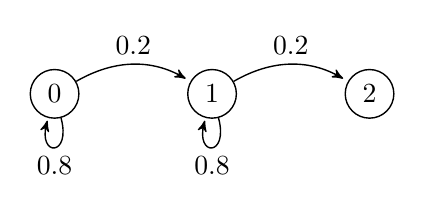
\begin{tikzpicture}[->,>=stealth',shorten >=2pt,line width=0.5pt,node distance=2cm]
\node [circle, draw] (n0) {0};
\node [circle , draw] (n1) [right of=n0] {1};
\node [circle , draw] (n2) [right of=n1] {2};
\path (n0) edge [bend left] node [above] {$0.2$} (n1);
\path (n1) edge [bend left] node [above] {$0.2$} (n2);
\path (n0) edge [loop below] node [below] {$0.8$} (n0);
\path (n1) edge [loop below] node [below] {$0.8$} (n1);
\end{tikzpicture}
\end{figure}

The story of this markov chain is that once we progress from node 0 to node 1, we can't move back to node 0. Similarly, once we're at node 1, we stay at node 1 until we reach node 2.

Let $T_{i}$ be the time spend at time $i$. It is easy to see that:
$$T = T_{1} + T_{2}$$

Now, we can think of progressing from one node to the next as a "success" with probability $p = 0.2$. The amount of time, or trials, it takes to progress to the next node is the number of failures + the final success. Therefore, $T_{1}, T_{2} \sim \text{FS}(0.2)$.

Thus, we can easily calculate $E(T)$:
$$E(T) = E(T_{1} + T_{2})$$
$$E(T) = E(T_{1}) + E(T_{2})$$
$$E(T) = 5 + 5 = 10$$

Similary, notice that $T_{1}$ and $T_{2}$ are independent; the number of times it took to get to node 1 doesn't affect how long it gets to node 2. Therefore:
$$\text{Var}(T) = \text{Var}(T_{1} + T_{2})$$
$$\text{Var}(T) = \text{Var}(T_{1}) + \text{Var}(T_{2})$$
$$\text{Var}(T) = 20 + 20 = 40$$

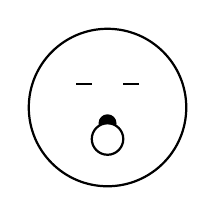
\begin{tikzpicture}
\draw[thick] (0cm,0cm) circle(1cm);
\draw[thick] (-0.4,0.3) -- (-0.2,0.3);
\draw[thick] (0.4,0.3) -- (0.2,0.3);
\draw [thick, fill=black] (0,-0.2) circle (0.1);
\draw [thick, fill=white] (0,-0.4) circle (0.2);
\end{tikzpicture}

\end{document}

